\section{HIERARQUIA ARITMÉTICA}
\label{sec:arithmetical_hierarchy}

Muitos outros problemas podem ser demonstrados equivalentes
(como oráculos)
ao problema da parada,
como o problema da correspondência de Post \cite[p.~214]{HopcroftUllman1979}.
Entretanto,
nem todos os problemas podem ser resolvidos com oráculos para a parada.
De fato, a mesma técnica que mostra que a parada é indecidível
pode ser usado para gerar um problema indecidível
para máquinas que usam o problema da parada como oráculo.

Defina
\simbolo{$L_u^n$}{Problema da parada, generalizado via oráculos}
\simbolo{$S_n$}{Problema da vacuidade, generalizado via oráculos}
\begin{align*}
    L_u^{n+1} &= \{ \langle M^{L_u^n}, x \rangle \mid M^{L_u^n} \text{ aceita } x \}, \\
    S_{n+1} &= \{ \langle M^{S_n} \rangle \mid L^{S_n}(M) = \emptyset \}.
\end{align*}
$L_u^{n+1}$ é o problema da parada
para máquinas de Turing que usam $L_u^n$ como oráculo;
$S_{n+1}$ é o problema da vacuidade
para máquinas de Turing que usam $S_n$ como oráculo.%
\footnote{
    Observe que,
    se definirmos $L_u^0 = S_0 = \emptyset$
    (ou algum conjunto recursivo qualquer),
    a fórmula é válida também para $n = 1$.
}
Podemos demonstrar por indução que $S_n$ é equivalente a $L_u^n$;
e, imitando o teorema da parada,
podemos mostrar que $L_u^{n+1}$ é indecidível para máquinas que usam $L_u^n$ como oráculo.

Defina
\simbolo{$\Sigma_n$}{Linguagens decidíveis usando um oráculo para $L_u^n$}
\begin{equation*}
    \Sigma_n = \{ L \mid L = L^{L_u^n}(M) \text{ para alguma máquina $M^{L_u^n}$ } \}.
\end{equation*}
Ou seja, $\Sigma_n$ é o conjunto das linguagens
que são decidíveis usando $L_u^n$ como oráculo.%
\footnote{
    Se usarmos a convenção de que $L_u^0 = \emptyset$,
    o conjunto $\Sigma_0$ é exatamente
    o conjunto das linguagens recursivamente enumeráveis
    (geralmente denotado por $\RE$).
}

O parágrafo anterior mostra que as linguagens $L_u^{n+1}$ e $S_{n+1}$
não pertencem a $\Sigma_n$.
Como, por definição,
ambas as linguagens $L_u^{n+1}$ e $S_{n+1}$ pertencem a $\Sigma_{n+1}$,
os conjuntos $\Sigma_n$ e $\Sigma_{n+1}$ são diferentes.
Temos, para todo $n$,
\begin{equation*}
    \Sigma_n \subset \Sigma_{n+1}.
\end{equation*}
Desta forma,
criamos uma hierarquia de problemas indecidíveis.%
\footnote{
    Em outras palavras,
    existem problemas ``mais indecidíveis'' que outros;
    é uma situação análoga à existência de infinitos de tamanhos diferentes.
}

Estes conjuntos também podem ser denotados por $\RE^{L_u^n}$;
as ``linguagens recursivamente enumeráveis que usam $L_u^n$ como oráculo''.
São as linguagens que são reconhecidas
pelo mesmo tipo de máquina usado para definir $\RE$,
mas agora equipadas com um oráculo para $L_u^n$.

Observe que,
de posse de um oráculo para $S_n$ (por exemplo),
ao ``programar'' uma máquina de Turing com esse oráculo,
podemos ``fingir'' que podemos usar qualquer linguagem de $\Sigma_n$ como oráculo
--- como esta linguagem possui um algoritmo que a resolve
usando o nosso oráculo $S_n$,
podemos substituir todas as chamadas àquele oráculo
por este algoritmo.
Abusando um pouco da notação,
podemos escrever
\begin{equation}
    \begin{aligned}
        \Sigma_0 &= \RE \\
        \Sigma_{n+1} &= \RE^{\Sigma_n}.
    \end{aligned}
    \label{eq:oracle_notation_abuse}
\end{equation}
A interpretação é que $\Sigma_{n+1}$ é o conjunto das linguagens
reconhecidas pelas mesmas máquinas de $\R$,
mas equipadas com um oráculo qualquer de $\Sigma_n$.
Como $S_n \in \Sigma_n$, esta nova definição inclui a definição anterior;
Como todas as linguagens de $\Sigma_n$
podem ser reconhecidas usando um oráculo para $S_n$,
qualquer linguagem de $\Sigma_{n+1}$
pode ser reconhecida usando apenas $S_n$
(basta fazer aquela troca de chamadas ao oráculo);
portanto as duas definições são equivalentes.
Usaremos esta notação novamente na seção~\ref{sec:polynomial_hierarchy},
mas indo direto à esta construção alternativa,
sem passar pela definição via $S_n$ primeiro.

Estendendo o exemplo do $\Sigma_n$,
podemos construir a hierarquia aritmética.%
\footnote{
    A hierarquia aritmética costuma ser caracterizada
    através de fórmulas de primeira ordem.
    Isto é,
    as linguagens de $\Sigma_n$ são as que podem ser descritas por
    \begin{equation*}
        \exists x_1 \forall x_2 \exists x_3 \dots Q x_n P(x, x_1, \dots, x_n)
    \end{equation*}
    em que o quantificador $Q$ depende da paridade de $n$.
    $\Pi_n$ é definido de maneira análoga,
    mas com o primeiro quantificador sendo um $\forall$.

    Esta construção alternativa é de \citeonline[p.~234]{DavisSigalWeyuker1994}.
}
\begin{definition}[Hierarquia aritmética]
    \begin{align*}
        \Sigma_0 &= \RE \\
        \Sigma_{n+1} &= \RE^{\Sigma_n} \\
        \Pi_n &= \ComplexityFont{co}\Sigma_n =
            \big\{ \{0, 1\}^* \backslash L \mid L \in \Sigma_n \big\} \\
        \Delta_n &= \Sigma_n \cap \Pi_n \\
    \end{align*}
\end{definition}

A hierarquia aritmética provê uma forma de ``medir''
o quão ``indecidível'' um problema é.
Intuitivamente, quão mais alto um problema está na hierarquia,
``mais indecidível'' este problema é.

Por exemplo, os problemas
\begin{equation*}
    \{ \langle M \rangle \mid L(M) = \Sigma^* \} \qquad \text{e} \qquad
    \{ \langle M \rangle \mid L(M) \text{ é finita } \}
\end{equation*}
são equivalentes a $S_2$ \cite[p.~211, 213]{HopcroftUllman1979},
portanto eles estão em $\Sigma_2 \backslash \Sigma_1$.
Em outras palavras,
de certa forma,
é ``mais difícil'' decidir se uma máquina de Turing aceita todas as palavras
do que decidir se ela aceita alguma.

Podemos mostrar que $\Sigma_n$ é um subconjunto próprio de $\Sigma_{n+1}$,
e que o mesmo vale para $\Pi_n$ e $\Pi_{n+1}$.
Temos
\begin{align*}
    \Pi_n \cup \Sigma_n & \subset \Delta_{n+1}, \\
    \Delta_{n+1} & \subset \Sigma_{n+1}, \\
    \Delta_{n+1} & \subset \Pi_{n+1}.
\end{align*}
Esta estrutura de inclusões
está esquematizada na figura~\ref{fig:arithmetical_hierarchy}.

\begin{figure}
    \centering
    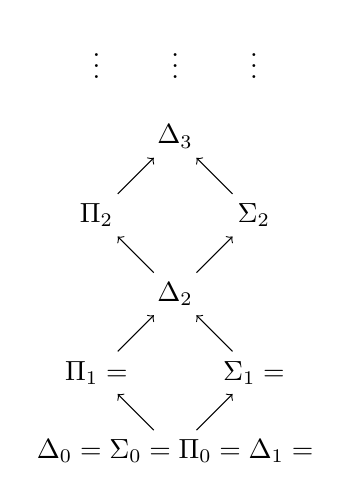
\begin{tikzpicture}
        \node (d1) at (0, 0) {$\Delta_0 = \Sigma_0 = \Pi_0 = \Delta_1 = \R$};
        \node (s1) at (1, 1) {$\Sigma_1 = \RE$};
        \node (p1) at (-1, 1) {$\Pi_1 = \coRE$};
        \node (d2) at (0, 2) {$\Delta_2$};
        \node (s2) at (1, 3) {$\Sigma_2$};
        \node (p2) at (-1, 3) {$\Pi_2$};
        \node (d3) at (0, 4) {$\Delta_3$};

        \begin{scope}[->]
            \draw (d1) -- (s1);
            \draw (d1) -- (p1);
            \draw (p1) -- (d2);
            \draw (s1) -- (d2);

            \draw (d2) -- (s2);
            \draw (d2) -- (p2);
            \draw (p2) -- (d3);
            \draw (s2) -- (d3);
        \end{scope}
        \node at (-1, 5) {$\vdots$};
        \node at (0, 5) {$\vdots$};
        \node at (1, 5) {$\vdots$};
    \end{tikzpicture}
    \caption[Estrutura de inclusões da hierarquia aritmética]{
        Estrutura de inclusões da hierarquia aritmética.

        As setas denotam inclusões estritas entre dois conjuntos.
    }
    \label{fig:arithmetical_hierarchy}
\end{figure}

Encontraremos uma estrutura de inclusões similar a esta
na seção~\ref{sec:polynomial_hierarchy}.
